\section{在 \t=1 处的分析}\label{teqone}

\begin{keytakeaways}
\begin{itemize}\setlength{\itemsep}{2pt}
  \item \textbf{物理图像}：沿 $x^1$ 拉伸后，把纽结问题约化为三维流形 $M_3=C\times\R_+$ 上的时间无关解，这类解保持四个超荷，结构因而大为简化。
  \item \textbf{数学工具}：把约化方程写成三个微分算符的交换条件与矩映射条件；前者在复规范变换下不变，后者只在 G-规范变换下不变，于是问题化归为 Hitchin 意义上的希格斯丛上的全纯数据。
  \item \textbf{主要结论}：正则 Nahm 极边界条件给出额外结构——$E$ 上一个处处不被 $\phi$ 稳定的全纯线子丛 $L$；在 $\R^2$ 上它由条件 $s\wedge\phi s=1$ 刻画（只固定 $\phi$ 的一个矩阵元）。
  \item \textbf{推广}：奇异磁单极子由 $s\wedge\phi s$ 的零点实现，零点重数即磁荷；对 $SU(N)$ 的主嵌入，$L$ 及其 $\phi$ 的幂次张成整个 $E$，构成一个旗。
\end{itemize}
\end{keytakeaways}

\subsection{若干预备知识}\label{preliminaries}

\begin{figure}
 \begin{center}
     % >>> 原文图 5（原稿第 11 页）
  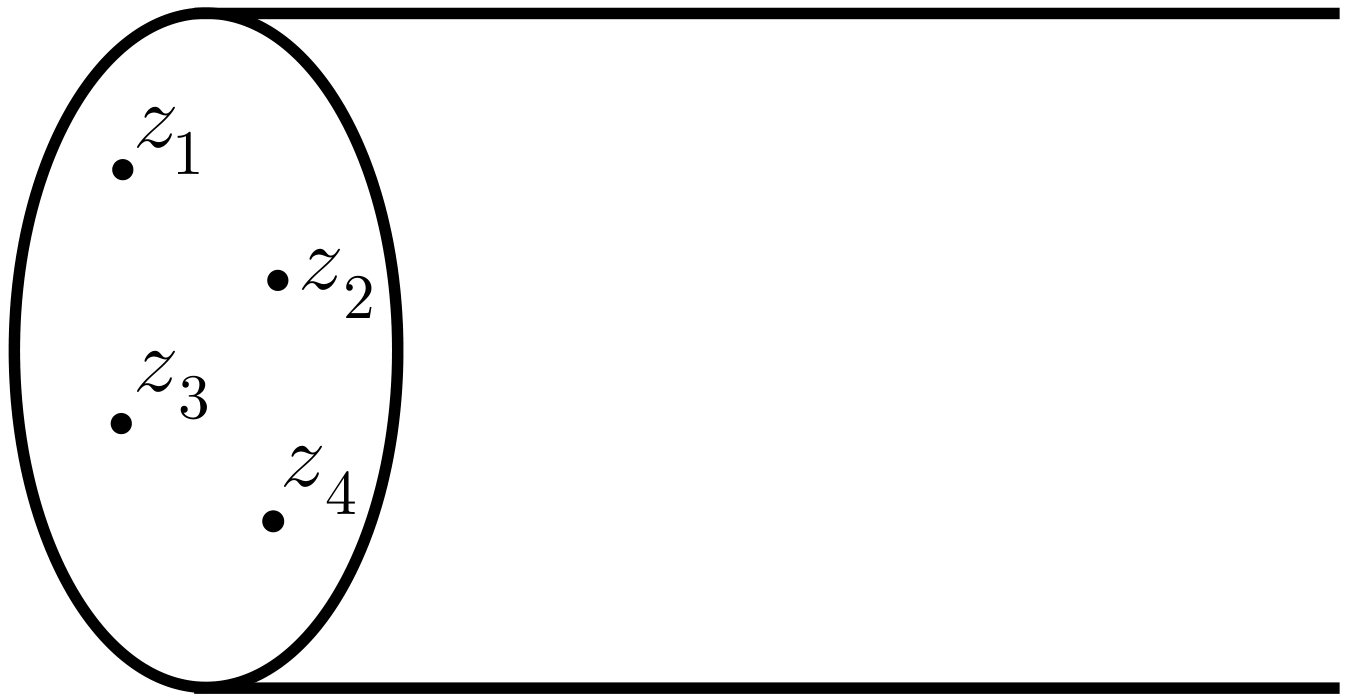
\includegraphics[width=3.5in]{figs/Fig05.png}
 \end{center}
\caption{\small  在时间无关的情形中，我们在三维流形 $M_3=C\times \R_+$ 上寻找解，其中 $C$（此处取为二维球面）是一个黎曼面。纽结被置于 $M_3$ 边界上的若干点处，此处标记为 $z_1,\dots,z_4$。（原稿第 11 页）}
 \label{redthree}
\end{figure}

正如引言中所解释的，在沿 $\MM=\R\times C\times\R_+$ 的第一个因子拉伸纽结之后，我们希望找出与第一个坐标（我们称之为 $x^1$）无关的解，也就是在三维流形\footnote{\label{confusion}
为避免混淆，我们作如下说明。本文中我们把 $\MM=\R\times C\times\R_+$ 按两种不同方式写成三维流形与一维流形的乘积：我们写
$\MM=W\times \R_+$ 而 $W=\R\times C$，但也写 $\MM=\R\times \Mthree$ 而
$\Mthree=C\times\R_+$。} $\Mthree=C\times \R_+$ 上满足约化方程的解。
这里 $C$ 是一个黎曼面（可以简单取为 $\R^2$），$\R_+$ 是半直线 $y\geq 0$。若存在纽结，我们取其支撑集为时间无关的形式 $\R\times z_i\times\{0\}$，其中 $z_i$ 是 $C$ 中的点，$\{0\}$ 是 $\R_+$ 的端点 $y=0$。图景见图~\ref{redthree}。

可由三维导出的解保持超过一般数量的超对称——确切地说，它们保持四个超荷——因此正如 \cite{fiveknots} 第 3.6 节所述，其结构会简化。在本文将会遇到的所有情形中，约化方程都可以用三个微分算符 $\D_i$（$i=1,2,3$）有效地描述。这些方程说的是：$\D_i$ 相互对易
\begin{equation}\label{commuting}[\D_i,\D_j]=0,\end{equation}
并满足矩映射条件
\begin{equation}\label{momentmap}\sum_{i=1}^3 [\D_i,\D_i^\dagger]=0,\end{equation}
其中 $\D_i^\dagger $ 是 $\D_i$ 在自然意义下的伴随。对易性约束 (\ref{commuting}) 在复值规范变换 $\D_i\to g\D_i g^{-1}$ 下不变，其中 $g$ 是取值于 $G_\C$ 的规范变换（$G_\C$ 是 $G$ 的复化）；而矩映射条件 (\ref{momentmap}) 只在取值于 $G$ 的规范变换下不变。使我们的问题变得可处理的关键在于：联立方程组的解模去 $G$-规范变换，等价于仅对易性约束 (\ref{commuting}) 的解模去 $G_\C$-规范变换。但对易性约束模去复规范变换后的解可以用全纯量来描述，因此有可能理解它们。
% [Tutor Note: 含糊点拨] 这里省略了证明，实为 Hitchin 方程/Kapustin-Witten 方程理论中的标准事实：先取 G_\C 规范把 [\D_i,\D_j]=0 化成全纯数据，再用 Hitchin 的稳定性与 Donaldson-Uhlenbeck-Yau 型定理求解矩映射，得到唯一的 G-规范等价类。此等价性并非对任意初值自动成立，前提是相应的希格斯丛满足（多）稳定性；作者在下文"我们期望可以由复规范变换求解"处再次使用了同一事实。

不同实例中的这一结构随 $\D_i$ 的构造而变，而后者依赖于 $\t$ 的选取，也依赖于我们在 $y=0$ 与 $y=\infty$ 处所设的边界条件。\cite{fiveknots} 中考虑的最基本情形是 $\t=1$（或 $-1$），且边界条件由 $\phi$ 中与边界相切的部分内的一个 Nahm 极给出。该边界条件令 $\phi_y$（即 $\phi$ 的法向部分）在 $y=0$ 处为零。若我们还要求 $\phi_y$ 在 $y\to\infty$ 时为零，则一个简单的消失性论证表明：在与 $x^1$ 无关的解中，$\phi_y$ 恒为零；类似地，$A_1$（即 $A$ 沿 $x^1$ 方向的分量）在三维解中也为零。一旦令 $\phi_y$ 与 $A_1$ 为零，方程便可写成上述形式，正如 \cite{fiveknots} 第 3.6 节\footnote{我们的记号与那里不同之处在于对坐标作了重新标号 $x^i\to x^{i+1}$（其目的是在范畴化时为新的时间坐标 $x^0$ "腾出空间"）。此外，为后文方便，我们以显然的方式置换了 $\D_i$。}中详细展示的那样，此时
\begin{align}\label{eqform} \D_1 & = \frac{D}{Dx^2}+i\frac{D}{Dx^3}    \cr
                                   \D_2 & = [\phi_2-i\phi_3,\,\cdot\,] \cr
                             \D_3 & = \frac{D}{Dy}-i[\phi_1,\,\cdot\,]  \end{align}
而矩映射条件成为
\begin{equation}\label{mmtmap}0=
\sum_{i=1}^3[\D_i,\D_i{}^\dagger]=F_{23}-[\phi_2,\phi_3]-D_y\phi_1.\end{equation}
 在写出这些公式时，我们简单地取 $C=\R^2$，坐标为 $x^2,x^3$。不过，引入复坐标 $z=x^2+ix^3$，并写 $\phi_2\d x^2+\phi_3\d x^3=\varphi \d z+\bar\varphi \d\bar z$，是有益的；我们还引入复联络 $\A_y=A_y-i\phi_1$ 用于沿 $y$ 方向的平行移动，并写 $\D_y=\d_y+[\A_y,\,\cdot\,]$。于是可以写成
\begin{align}\label{neqform} \D_1 & =2\frac{D}{D\bar z} \cr
                                                              \D_2 & = 2[\varphi,\,\cdot\,]\cr
                                                               \D_3& = \frac{\D}{\D y}. \end{align}
以这种写法，$\D_i$ 在任意黎曼面 $C$ 上都有意义，其中 $D/D\bar z$ 理解为 $\bar\partial $ 算子，$\varphi$ 为 $C$ 上的一个 $(1,0)$-形式。
% [Tutor Note: 约定差异] 与 \cite{fiveknots} 比对时须注意脚注中的坐标重标号 x^i\to x^{i+1} 以及对 \D_i 的置换；此外 z=x^2+ix^3 的选取使 \partial_z 与 \partial_{\bar z} 的归一化相差因子 2，故 \D_1=2D/D\bar z 中的系数 2 依赖于该约定。复联络写成 \A_y=A_y-i\phi_1（而非 +i\phi_1），这个符号决定了 \D_3 中与 \phi_1 的对易子项的符号，进而决定 \phi_1 与 A_y 在希格斯丛复结构中的角色。

正如保持四个超荷的几何所预期的那样，对易性约束 $[\D_i,\D_j]=0$ 可以由一个超势导出，即
\begin{equation}\label{superone}\W= \frac{1}{4\pi i}\int_{C\times \R_+}\Tr\,\varphi \F_{y\bar z},\end{equation}
其中 $\F_{y\bar z}=[\D_y,D_{\bar z}]$。更准确地说，在变分 $\W$ 以导出条件 $[\D_i,\D_j]=0$ 时，应当要求 $A$ 在 $y=0$ 处的变分为零。否则 $\W$ 的变分会包含 $y=0$ 处额外的 delta 函数项。
% [Tutor Note: 易错点] 超势变分在带边流形上会产生边界项：\delta\W 除给出 [\D_i,\D_j]=0 外，还给出正比于 \int_{y=0}\Tr(\varphi\,\delta A) 的项。只有限制 \delta A|_{y=0}=0 时，[\D_i,\D_j]=0 才恰为超势的临界条件；否则须把该边界项一并处理（这正是后文把 Nahm 极边界条件视为对变分原理的约束的原因）。

方程 $[\D_i,\D_j]=\sum_i[\D_i,\D_i{}^\dagger]=0$ 在 \cite{KW} 中被称为推广的 Bogomolny 方程；实际上，这些方程是 Nahm、Hitchin 与 Bogomolny 方程的混合体。若丢掉对 $z$ 的依赖，它们约化为 Nahm 方程；若丢掉对 $y$ 的依赖，它们约化为 Hitchin 方程；若令 $\varphi=0$，则约化为 Bogomolny 方程。这不仅仅是一个类比：我们可以借用 Nahm、Hitchin 或 Bogomolny 方程模空间理论中的标准策略。

对固定的 $y$，方程 $[\D_1,\D_2]=0$ 定义了 Hitchin 意义上的一个希格斯丛 $(E,\varphi)$。$\D_1$ 与 $\D_2$ 同 $\D_3$ 对易这一事实只意味着：在复值规范变换的意义下，该希格斯丛与 $y$ 无关。当我们特殊到 $C=\R^2\cong \C$ 时，便得到 $\C$ 上的一个希格斯丛，它可以理解为 $\CP^1=\C\cup \infty$ 上的希格斯丛，可能在无穷远处带有奇点。这一情形将在第~\ref{simvar}~节中考虑。希格斯丛的奇点还有另一种自然的产生方式。如 \cite{fiveknots} 第 6 节所述，可以纳入支撑在 $\MM$ 中余维二维子流形上的曲面缺陷。把它们取为 $\R\times q_i \times \R_+$ 的形式（其中 $q_i$ 是 $C$ 中的点），上面概括的构造仍然适用，而希格斯丛在点 $q_i$ 处获得奇点。我们在第~\ref{mondr}~节中考虑这一情形。

额外的结构来自 $y=0$ 与 $y=\infty$ 处的边界条件。我们将在第~\ref{bc}~节中讨论 $y=0$ 处 Nahm 极的后果。与 Nahm 方程的类比将会有用：对 $C$ 中的任一给定点，我们可以从对易对 $\D_2$,$\D_3$ 中提取某些全纯数据。由于 $\D_2$,$\D_3$ 与 $\D_1$ 对易，这些数据在全纯意义下（或在存在奇点时在亚纯意义下）随 $C$ 变化。

最后，与 Bogomolny 方程的类比将帮助我们理解解的物理内容，尤其是当我们在 $y\to\infty$ 时开启规范对称性破缺时。的确，对易对 $\D_1$,$\D_3$ 中的全纯数据，类似于在 Bogomolny 方程的解中指定 BPS 磁单极子位置的那些数据。

\subsection{边界条件}\label{bc}
我们的下一个任务是分析边界条件，首先在没有奇异磁单极子的情形下。$\t=1$ 时的模型解 (\ref{nahmpole}) 在 $\D_2$ 与 $\D_3$ 中有奇点，但在 $\D_1$ 中没有奇点，这仅仅是因为 $\D_1$ 不含标量场。对 $ \frak g = \frak{su}(2)$，取李代数元素 $\ct$ 的标准选取，该解显式为
\begin{equation}\label{burg}
\varphi = \frac{1}{y} \begin{pmatrix} 0 & 1 \cr 0 & 0\end{pmatrix},
\qquad A_{\bar z}=0, \qquad \A_y = \frac{1}{2y} \begin{pmatrix} 1 & 0 \cr 0 & -1\end{pmatrix}.
\end{equation}
我们在此认为这些矩阵作用在秩为二的平凡复向量丛 $E\to \R^2\times\R_+$ 的纤维上。对 $G=SO(3)$、在一般的黎曼面上，把 $E$ 定义为秩二的丛可能存在整体障碍，这时人们会转而考虑相应的伴随丛 $\ad(E)$。由于我们的考虑沿黎曼面 $C$ 是局域的，改用伴随表示重新表述不会有太大变化，我们将略过这一点。


解 (\ref{burg}) 可以写成
\begin{equation}\label{nolf} \varphi= g\varphi_1 g^{-1},
~~ \D_y=g\frac{\d}{\d y}g^{-1} \end{equation}
其中
\begin{equation}\label{zolf} \varphi_1=\begin{pmatrix} 0 & 1\cr 0 & 0 \end{pmatrix}\end{equation}
而 $g$ 是一个在 $y=0$ 处奇异的 $G_\C$ 值规范变换
\begin{equation}\label{singgauge}
g =\begin{pmatrix} y^{-1/2} & 0 \cr 0 & y^{1/2} \end{pmatrix}.
\end{equation}
换言之，该解是由平凡解 $\varphi=\varphi_1,$ $A_{\bar z}=\A_y=0$ 经复值规范变换 $g$ 得到的。

我们希望考虑在 $y=0$ 附近、在相差一个规范变换的意义下看起来像模型解的那些解。我们希望用远离边界处的希格斯丛数据 $(E,\varphi)$ 来表达这一约束。为此，考察规范丛 $E$ 的一个局部全纯截面 $s$ 在沿 $y$ 方向平行移动下不变时的行为，是有用的。我们将先对模型解非常具体地做这一计算，然后再辨认哪些特征在更一般的情形下仍然成立。

设 $s$ 是规范丛 $E$ 的一个截面，满足
\begin{equation}\label{onurf}\frac{\D s}{\D y}=0.\end{equation}
由于 $\D/\D y= g (\d/\d y) g^{-1}$，该方程的解具有 $s= gs_0$ 的形式，其中 $s_0$ 与 $y$ 无关。因此通解具有形式
\begin{equation}\label{wurf} s=\begin{pmatrix} a y^{-1/2}\cr b y^{1/2}\end{pmatrix},\end{equation}
其中 $a,b$ 为常数。特别地，$E$ 中一个一般的向量沿 $y$ 方向平行移动到 $y=0$ 时会按 $y^{-1/2}$ 发散。存在一个一维子空间，由满足 $\D s/\D y=0$ 且在 $y\to 0$ 时实际按 $y^{1/2}$ 消失的那些解组成。该子空间简单地由条件 $a=0$ 刻画。

对任意固定的 $y>0$，我们把 $E\to C\times \R_+$ 到 $C\times \{y\}$ 的限制记作 $E_y$。用 $\D_y$ 作平行移动给出所有 $y$ 的 $E_y$ 之间的自然等同，我们就把 $E_y$ 视为 $C$ 上的丛并简单地记作 $E$。类似地，$\varphi$ 到 $C\times y$ 的限制在 $\D_y$ 平行移动的意义下与 $y$ 无关。于是通过限制到 $C\times y$，我们得到希格斯丛 $(E,\varphi)\to C$。

$E$ 的"小"截面——即满足 $\D s/\D y=0$ 且在 $y\to 0$ 时消失的解 $s$——生成一个秩一子丛 $\L\subset E$。在模型解中，它简单地就是 $E$ 中形如 $\begin{pmatrix}0\cr b\end{pmatrix}$ 的截面所构成的子丛。$\L$ 是 $E\to C$ 的全纯子丛；$\L$ 的一个截面若被 $\D_1=2\,D/D\bar z$ 湮灭，则它是全纯的。具体地说，在模型解中，$\L$ 的截面 $\begin{pmatrix}0\cr b\end{pmatrix}$ 全纯当且仅当 $b$ 是 $z$ 的全纯函数。

$\L$ 全纯的根本原因在于：由于 $[\D_2,\D_3]=0$，我们可以要求 $\D_3s=0$ 的小解同时也被 $\D_2=2D/D\bar z$ 湮灭。然而，我们不能同时要求小解被 $\varphi=\D_1/2$ 湮灭。这一点从上面的公式看很清楚：在模型解中，$\varphi$ 湮灭一个向量当且仅当其下分量为零，而不是当其上分量为零。

为衡量 $\L$ 不是 $\varphi$-不变的程度，可以如下进行。若 $\L$ 是一个平凡线丛（在我们的应用中将是如此），则可选取 $\L$ 的一个处处非零的截面 $s$。对我们的模型解，只需取 $s=\begin{pmatrix} 0 \cr 1\end{pmatrix}$。然后我们定义
\begin{equation}\label{smallexp}  \kappa= s\wedge \varphi s.  \end{equation}
对模型解，我们看到 $\kappa=1$，特别地
$\kappa$ 处处非零。$\kappa$ 非零意味着 $\varphi s $ 不是 $s$ 的倍数，因此 $\L$ 不满足在乘以 $\varphi$ 下不变这一性质。
（若把 $\R^2$ 换成一般的黎曼面 $C$，可能无法选取整体非零的 $s$，但人们仍可选取 $\L$ 的一个局部截面 $s$，并通过计算 $\kappa=s\wedge \varphi s$ 来度量 $\L$ 不是
$\varphi$-不变的程度。只要 $s$ 非零，$\kappa$ 是否为零就与 $s$ 的选取无关。）

对模型解成立的三条基本性质，对任何带正则 Nahm 极的解仍然成立，因为它们不受 $y \to 0$ 时 $\D_y$ 与 $\varphi$ 的次领头行为的影响：
\begin{itemize} \item $E$ 中一个一般的向量沿 $y$ 方向平行移动到
$y=0$ 时会按 $y^{-1/2}$ 发散。 \item  那些平行移动到 $y=0$ 时实际消失的截面 $s$ 张成一个秩 1 的全纯子丛  $\L\subset E$。  \item
最后，我们不能同时要求一个小截面被 $\varphi=\D_1/2$ 湮灭。相反，在 $y=0$ 附近可由模型解逼近的解中，$\varphi$ 在 $C$ 中的任何点处都不湮灭小截面。\end{itemize}
% [Tutor Note: 物理图像] 这三条性质合起来就是"保留结构群"的图像：Nahm 极把 G_\C 结构群约化为一个抛物子群，\L 是该抛物结构中的最小子丛，\kappa=s\wedge\varphi s 则是这个抛物结构偏离 \varphi-稳定性的量度。因此"希格斯丛 + 处处非 φ-稳定的线子丛"正是 Nahm 极边界条件所编码的全纯数据，而不是任意的希格斯丛。

因此，带正则 Nahm 极（$y\to 0$）的完整方程的解所给出的并不仅仅是希格斯丛 $(E,\varphi)$。更确切地说，还存在某种额外的结构：$E$ 被赋予一个全纯线子丛 $\L$，它在任何地方都不被 $\varphi$ 稳定。在 $\R^2$ 上，$\L$ 必然是平凡的，因此我们可以简单地说：$E$ 存在一个处处非零的全纯截面 $s$，满足 $s \wedge \varphi s =1$。注意这一条件远不足以确定 $\varphi$。若 $s=\begin{pmatrix}0\cr 1\end{pmatrix}$，则条件 $s\wedge \varphi s=1$ 只固定 $\varphi$ 的右上角矩阵元，对其余矩阵元不加任何条件。之所以只固定 $\varphi$ 的一个矩阵元（用 $s$ 表示），是因为当我们作一个在 $y\to 0$ 时行为如 (\ref{singgauge}) 的规范变换时，$\varphi$ 获得的奇点只依赖于它的右上角矩阵元。在适当的情形下（亏格更高的黎曼面 $C$ 上，或在存在下面即将引入的奇异磁单极子的 $\R^2$ 上），可以存在由三元组 $(E,\varphi,\L)$ 构成的非平凡模空间，其中 $E$ 与 $\L$ 固定而只有 $\varphi$ 变化。这一点将在第~\ref{opbranes}~节中说明。

对任何三元组 $(E,\varphi,\L)$，我们期望完整方程组可以通过一个复规范变换求解。假设给定一个与 $y$ 无关的希格斯丛 $(E,\varphi)$，以及一个处处不被 $\varphi$ 稳定的全纯子丛 $\L\subset E$。在以 $\varphi s$ 与 $s$ 给出的 $E$ 的基中，我们作规范变换 (\ref{singgauge})。这将重现 $y=0$ 处的 Nahm 极奇点，但一般而言它不会给出矩映射条件 (\ref{mmtmap}) 的解。通过进一步作光滑的复规范变换，人们有望得到矩映射条件的解。
% [Tutor Note: 含糊点拨] "有望"（one can hope）背后是 Hitchin-Kapustin-Witten 的定理：给定希格斯丛若满足稳定性，则存在唯一的光滑复规范变换使矩映射为零；若不稳定，则只能得到"近似"解或需要引入额外的奇异结构。作者此处未验证稳定性条件，后文讨论库仑分支参数 \vec\ca 与纽结标号 R^\vee 的容许范围时才间接涉及这一限制，阅读时应留意。

\subsubsection{加入奇异磁单极子}\label{addsing}

为在边界处加入奇异磁单极子，我们需要用更一般的奇异解来替换 Nahm 模型解，该解见 \cite{fiveknots} 第 3.6 节。让我们考虑单个奇异磁单极子的情形，它位于 $y=z=0$。模型解在 $y\to 0$ 且 $z\not=0$ 时具有与前面相同的奇点，但在 $y=z=0$ 附近具有更复杂的形式。它可以由对易性约束的一个解经复值规范变换得到（该变换在 \cite{fiveknots} 中有明确描述），该解为
\begin{equation}\label{solcom} \varphi=
\begin{pmatrix} 0 & z^k\cr 0 & 0 \end{pmatrix}, ~~A_z=\A_y=0.
\end{equation}
为用我们现在的语言表达这一点，$\L$ 仍然由这样的截面张成：在规范 (\ref{solcom}) 中它们是
$s=\begin{pmatrix} 0 \cr 1 \end{pmatrix}$ 的倍数；这是因为 $g$ 在 $y\to 0$ 时具有与前面类似的行为。现在我们得到
\begin{equation} s\wedge\varphi s = z^k.\end{equation}
$s\wedge\varphi s$ 的零点被解释为奇异磁单极子的位置，其重数即为磁荷。这一解释立刻提示了含多个奇异磁单极子的解应当意味着什么。我们考虑由希格斯丛 $(E,\varphi)$ 及一个一般地不是 $\varphi$-不变的全纯子丛 $\L\subset E$ 所描述的解。若
\begin{equation}\label{olcomtwo} s\wedge \varphi s =\prod_{a=1}^s(z-z_a)^{k_a},\end{equation}
则我们说该解在位置 $z_a$ 处有磁荷为 $k_a$ 的奇异磁单极子。人们希望能证明：给定这样的数据，存在唯一解，它在每个 $z=z_a$ 附近的奇性与奇异模型解一致。
% [Tutor Note: 物理图像] 磁单极子的"位置"是 s\wedge\varphi s 的零点这一事实，说明奇异磁单极子并不作为独立的场存在，而是希格斯丛数据 (E,φ,L) 的奇点；电荷 k_a 即是零点重数，这也解释了为何对偶群 G^\vee 的表示 R^\vee 的维数会成为磁荷——它正是 s\wedge\varphi s 在纽结处的零点阶数。

尽管本文主要考虑 $\frak{su}(2)$，我们可以很容易地把这些陈述推广到更一般的李代数。为简单起见，取 $G=SU(N)$ 并把 $E$ 看作秩为 $N$ 的复向量丛。考虑基于 $\frak{su}(2) \to \frak{su}(N)$ 的主嵌入的 Nahm 极。$\ct_3$ 的本征空间（在 $\frak{su}(N)$ 的基本 $n$ 维表示中）是一维的，而由在 $y \to 0$ 时尽可能快地衰减的截面定义了一个线丛 $\L$。对 $\L$ 的唯一约束是：在奇异磁单极子位置之外，
\begin{equation}
 \L \oplus \varphi \L \oplus  \cdots \oplus \varphi^{n -1} \L = E
\end{equation}
当我们特殊到 $C=\R^2\cong \C$ 时，可以用 $E$ 的一个特定截面 $s$（在重新标度意义下定义）来定义线子丛 $\L$，使得截面 $s, \varphi s, \cdots,\varphi^{N-1}s$ 线性无关。这一约束在奇异磁单极子所在处按其磁荷的方式被放宽。用 $\varphi$ 的矩阵元的零点给出的等价描述见 \cite{fiveknots} 式 (3.59)。
% [Tutor Note: 原文笔误] 本段先设 G=SU(N)、E 秩为 N，但接着写"基本 n 维表示"并把分解式写成 \L\oplus\varphi\L\oplus\cdots\oplus\varphi^{n-1}\L=E；按主嵌入的维数应为 N（下文也确实写成 \varphi^{N-1}s）。原文如此，n 疑为 N 之笔误，译文未改动公式。

这可以推广到 $y=0$ 处一般 Nahm 极的情形，不必与 $\frak{su}(2)$ 的主嵌入相联系。（本文不研究这一推广。）一般地，对 $y\to 0$，存在按 $y$ 的整数或半整数幂增长的局部截面。
通过考察在 $y \to 0$ 时至多按给定幂 $y^{(n-N)/2}$ 增长的局部截面，可以在 $E$ 上定义一个全纯子丛的旗 $E_n$。显然，$E_{n+1} \subset E_n$；又有  $E_0=E$，且对足够大的 $n$ 有 $E_n=0$。乘以 $y^{-(n-N)/2}$ 后，$E_n$ 中一个一般的向量在 $y \to 0$ 时具有有限极限，而此极限是 $\ct_3$ 的、本征值为 $(N-n)/2$ 的本征向量。该映射的核为 $E_{n+1}$；因此 $y \to 0$ 的极限把商空间 $E_n/E_{n+1}$ 与 $\ct_3$ 的本征空间等同起来。乘以 $\varphi$ 给出映射 $E_n \to E_{n-2}$。由于 $\varphi \sim \frac{\ct_+}{y}$，全纯映射 $\phi_n : E_n/E_{n+1} \to E_{n-2}/E_{n-1}$ 可以等同于 $\ct_+$ 在 $\ct_3$ 的本征空间上的作用。
